% IEEE Conference Paper Template
% GitaGraph: Ontology-Driven AI System for Bhagavad Gita Philosophical Navigation
\documentclass[conference]{IEEEtran}
\IEEEoverridecommandlockouts

\usepackage[utf8]{inputenc}
\renewcommand{\ttdefault}{cmtt}
\usepackage{cite}
\usepackage{amsmath,amssymb,amsfonts}
\usepackage{algorithmic}
\usepackage{graphicx}
\usepackage{textcomp}
\usepackage{xcolor}
\usepackage{booktabs}
\usepackage{array}
\usepackage{multirow}
\usepackage{url}
\usepackage{hyperref}
\usepackage{listings}
\usepackage{enumitem}
\setlength{\abovecaptionskip}{4pt}
\setlength{\belowcaptionskip}{2pt}

\lstset{
  basicstyle=\ttfamily\footnotesize,
  breaklines=true,
  frame=single,
  numbers=left,
  numberstyle=\tiny\color{gray},
  keywordstyle=\color{blue},
  commentstyle=\color{green!50!black},
  stringstyle=\color{orange}
}

\def\BibTeX{{\rm B\kern-.05em{\sc i\kern-.025em b}\kern-.08em
    T\kern-.1667em\lower.7ex\hbox{E}\kern-.125emX}}

\begin{document}

\title{GitaGraph: An Ontology-Driven Knowledge-Based AI System\\
for Philosophical Navigation of the Bhagavad G\={i}t\={a}}

\author{
\IEEEauthorblockN{Hariom Rajput, Ayushi Choyal, Ravi Kant Gupta, Shouryavi Awasthi}
\IEEEauthorblockA{\textit{Department of Computer Applications}\\
\textit{National Institute of Technology, Kurukshetra}\\
Kurukshetra, Haryana, India\\
\{524110006, 524410017, 524410027, 524410028\}@nitkkr.ac.in}
}

\maketitle

%-----------------------------------------------------------------------
\begin{abstract}
The Bhagavad G\={i}t\={a}, a foundational text of Indian philosophy comprising
700 Sanskrit verses across 18 chapters, presents a rich domain for knowledge
representation and semantic reasoning. Readers approaching the text face significant
challenges: navigating non-linear philosophical dependencies, resolving contradictions
between yoga paths, and constructing personalized study sequences from over 701 verses
without pedagogical guidance. Existing digital resources treat the G\={i}t\={a} as a
static corpus, offering keyword search but no structured reasoning or inference.

This paper presents \textbf{GitaGraph}, a modular knowledge-based AI system that
models the Bhagavad G\={i}t\={a} as a semantic knowledge graph. The system integrates
six classical AI techniques: (1) an OWL~2 ontology encoding 658 RDF triples over 16
classes and 9 object properties—including transitive and symmetric OWL axioms—across
30 annotated verses; (2) four graph search algorithms (BFS, DFS, A*, IDDFS) operating
over a 61-node, 175-edge philosophical concept graph; (3) an 8-rule forward-chaining
expert system with SPARQL-backed competency queries; (4) a backtracking Constraint
Satisfaction Problem (CSP) solver with MRV heuristic and forward checking to generate
5-session personalized study plans; and (5) a multi-modal uncertainty handler combining
MYCIN certainty factors (peak CF = 0.9991), fuzzy yoga-path membership functions, and
non-monotonic belief revision across three commentary traditions.

Experimental results demonstrate that A* search produces optimal 3-hop paths from
philosophical concepts to \textit{Mok\d{s}a}, the CSP planner satisfies all 7 hard
constraints in under 0.3 seconds, and MYCIN reasoning achieves strong evidence
aggregation across conflicting commentaries. The system is deployed as an
interactive Streamlit application and a REST API, serving as both a research
prototype and an educational tool for AI-assisted Sanskrit philosophical analysis.
\end{abstract}

\begin{IEEEkeywords}
knowledge graph, OWL ontology, SPARQL, A* search, constraint satisfaction, MYCIN
\end{IEEEkeywords}

%=======================================================================
\section{Introduction}

\subsection{Background and Motivation}

The Bhagavad G\={i}t\={a} (\textit{Song of the Divine}) is one of the most
widely studied philosophical texts in the world, embedded within the
Mah\={a}bh\={a}rata epic. Comprising 700 \'{s}lokas (verses) in 18 chapters
(\textit{adhy\={a}yas}), it presents a systematic dialogue between the warrior
prince Arjuna and his charioteer Krishna, covering epistemology, ethics, cosmology,
and four paths of liberation (\textit{yoga})—Karma, J\~{n}\={a}na, Bh\={a}na, and
Dhy\={a}na Yoga.

Despite its philosophical depth and global readership exceeding 100 million
practitioners~\cite{flood1996introduction}, the text poses serious navigational
challenges. Its verses are not arranged in a sequential pedagogical order; rather,
philosophical concepts form a directed acyclic graph (DAG) of prerequisites,
contrasts, and causal chains. A reader experiencing anxiety may need Verse~2.47
(\textit{karmaṇy evādhikāras te}—``focus only on action, not fruits''), but
discovering this connection requires traversing the conceptual dependency from
\textit{Anxi\={a}t\={a}} through \textit{Ni\d{s}k\={a}ma Karma} to the relevant
verse—a non-trivial knowledge graph traversal.

Classical AI offers a natural toolset for this problem: ontologies encode
philosophical taxonomy; graph search identifies shortest conceptual paths; expert
systems map reader profiles to canonical interpretations; and uncertainty quantification
resolves inter-commentary conflicts. Yet no existing system applies this comprehensive
classical AI stack to Sanskrit philosophical text navigation.

\subsection{Limitations of Existing Approaches}

Current digital G\={i}t\={a} resources exhibit four key limitations:

\textbf{Keyword-only retrieval:} Platforms such as the Bhagavad Gita App and
vedabase.io implement string-matching search, returning verses that contain keywords
but ignoring philosophical relationships. A query for ``anger'' does not surface
the causal chain \textit{K\={a}ma} $\to$ \textit{Krodha} $\to$ \textit{Moha} $\to$
\textit{Buddhin\={a}\'{s}a}.

\textbf{No structured knowledge representation:} Existing projects (e.g., DBpedia
G\={i}t\={a} entries) use flat triple stores without OWL axioms, preventing transitive
and property-chain inference. The entailment that ``one who teaches NishkamaKarma
spiritually progresses toward Moksha'' (via the property chain
\texttt{teaches $\circ$ leadsTo $\to$ spirituallyProgressesTo}) cannot be derived.

\textbf{No personalized study planning:} No system addresses the constraint satisfaction
problem of generating study plans satisfying chapter-coverage, prerequisite-ordering,
and goal-specific constraints simultaneously.

\textbf{No uncertainty quantification:} The G\={i}t\={a} has been interpreted by
hundreds of \={a}c\={a}ryas (teachers); three dominant traditions—Advaita (\'Sankara),
Vi\'si\d{s}\d{t}\={a}dvaita (R\={a}m\={a}nuja), and Dvaita (Madhva)—assign different
weight to verses. No digital tool models this disagreement using certainty factors or
fuzzy membership.

\subsection{Objectives and Contributions of this Project}

This project makes the following contributions:

\begin{itemize}[leftmargin=*]
  \item \textbf{OWL~2 Ontology Design:} A formally verified Bhagavad G\={i}t\={a}
        ontology with 16 classes, 9 object properties (including \texttt{owl:TransitiveProperty},
        \texttt{owl:SymmetricProperty}, and property chain axioms), encoding 658 RDF
        triples over 30 verses and 24 concepts.

  \item \textbf{Multi-Algorithm Graph Search:} Four graph search algorithms (BFS, DFS,
        A*, IDDFS) operating on a 61-node, 175-edge philosophical knowledge graph, with
        an admissible A* heuristic proven to never overestimate distance to
        \textit{Mok\d{s}a}.

  \item \textbf{Production-Rule Expert System:} An 8-rule forward-chaining system with
        specificity-based conflict resolution and 8 SPARQL Competency Questions (CQs)
        that prove ontological completeness.

  \item \textbf{CSP Study Planner:} A 5-variable CSP solver with backtracking, MRV
        heuristic, and forward checking, satisfying 7 hard constraints for personalized
        verse scheduling.

  \item \textbf{Multi-Modal Uncertainty Handler:} Integration of MYCIN certainty factors,
        fuzzy yoga-path membership, and non-monotonic belief revision.

  \item \textbf{Deployable System:} An interactive Streamlit application (8 pages) and
        Flask REST API demonstrating all six AI modules.
\end{itemize}

%=======================================================================
\section{Related Work}

\subsection{Knowledge Representation for Ancient Texts}

Noy and McGuinness~\cite{noy2001ontology} established foundational guidelines for
ontology development, which have been applied to historical corpora. Nurmikko-Fuller
and Page~\cite{nurmikko2016linked} demonstrated linked data approaches for musicological
corpora; analogous challenges arise in Sanskrit philosophy—complex taxonomies,
polysemic terms, and multi-tradition interpretations. The W3C OWL~2 specification
\cite{mcguinness2004owl} enables formal reasoning via DL-based reasoners, providing
inference capabilities absent in flat keyword systems.

For Sanskrit texts specifically, Goyal et al.~\cite{goyal2012sanskrit} surveyed NLP
approaches to Sanskrit analysis, noting that computational treatment is challenging
due to the rich morphology of P\={a}{\d{n}}ini's grammar. However, knowledge-graph
approaches that abstract over surface form offer a complementary path. No prior work
has constructed a formally verified OWL ontology for the Bhagavad G\={i}t\={a}.

\subsection{Semantic Web and Knowledge Graphs}

Bizer et al.~\cite{bizer2009linked} established principles for Linked Open Data,
showing how RDF triples enable cross-domain knowledge integration. SPARQL~\cite{harris2013sparql}
provides a standard query language over RDF graphs that supports pattern matching,
optional clauses, and aggregation—capabilities exploited in our 8 Competency Question
framework. Horrocks~\cite{horrocks2008ontologies} reviewed the state of ontological
reasoning, noting that OWL~2 EL and QL profiles balance expressivity with tractable
inference—our ontology targets the OWL~2 DL profile for maximum expressiveness.

\subsection{Graph Search in Knowledge Systems}

Hart, Nilsson, and Raphael's seminal work~\cite{hart1968formal} formalized the
A* algorithm and admissibility conditions for heuristic functions. In knowledge
graph settings, Bollacker et al.~\cite{bollacker2008freebase} demonstrated large-scale
structured knowledge navigation. Wang et al.~\cite{wang2014knowledge} reviewed
embedding-based KG completion—distinct from our symbolic search approach, which
prioritizes interpretability and formal guarantees over statistical coverage.
IDDFS was introduced by Korf~\cite{korf1985depth} as a space-efficient alternative
to BFS for deep search problems, which we apply to verse chains of unknown depth.

\subsection{Expert Systems and Production Rules}

The MYCIN system~\cite{shortliffe1976computer} pioneered certainty-factor reasoning
in expert systems, using the combination formula $CF(A,B) = CF_1 + CF_2(1-CF_1)$
for independent confirming evidence. Subsequent work by Buchanan and
Shortliffe~\cite{buchanan1984rule} systematized production-rule knowledge bases with
conflict resolution strategies. Our expert system inherits this lineage, applying
specificity-ordered conflict resolution to 8 reader-profile rules.

For natural language competency questions over ontologies, the approach of
Grüninger and Fox~\cite{gruninger1995methodology} provided formal methodology. We
adopt their CQ framework to validate that our ontology captures the semantic
commitments of G\={i}t\={a} philosophical discourse.

\subsection{Constraint Satisfaction and Study Planning}

Kumar~\cite{kumar1992algorithms} surveyed backtracking algorithms for CSPs, including
the MRV (Minimum Remaining Values) heuristic—also called ``fail-first''—which selects
the variable with the smallest domain to minimize backtracking. Haralick and
Elliott~\cite{haralick1980increasing} formalized forward checking as domain
propagation. In educational planning, Freuder~\cite{freuder1982sufficient} established
theoretical sufficiency conditions for constraint propagation in scheduling problems,
directly applicable to our 5-session verse assignment problem.

\subsection{Uncertainty in Knowledge Systems}

Zadeh's foundational paper~\cite{zadeh1965fuzzy} introduced fuzzy sets as a formal
model of gradual membership, enabling non-crisp set operations. Applied to yoga-path
classification, fuzzy membership captures the documented fact that many G\={i}t\={a}
verses address multiple paths simultaneously (e.g., Verse~6.47 is simultaneously
canonical for Bh\={a}na, Dhy\={a}na, and J\~{n}\={a}na Yoga). Reiter's default
logic~\cite{reiter1980logic} provides the formal foundation for non-monotonic belief
revision—our system implements a simplified version where new verse readings trigger
retraction of prior defaults.

\subsection{AI in Education and Personalised Learning}

AI-driven study planners have been applied to MOOC recommendation
(Khanal et al., 2020) and intelligent tutoring systems (VanLehn~\cite{vanlehn2011relative}),
where constraint-based models schedule learning objectives while satisfying
prerequisite graphs. Our CSP formulation mirrors this paradigm but targets
philosophical verse sequences rather than skill trees. Chen et al.~\cite{chen2018kgtutor}
proposed knowledge-graph tutoring systems that route learners along concept paths—the
closest prior work to our graph-search module—but did not apply symbolic search
algorithms with formal admissibility guarantees.

\subsection{Computational Philology and Digital Humanities}

The DHARMA project~\cite{dharma2020} and GRETIL corpus apply TEI/XML encoding
to Sanskrit texts, establishing metadata standards for verse annotation. Hellwig
and Nehrdich~\cite{hellwig2018sanskrit} demonstrated dependency parsing for
Classical Sanskrit using neural taggers. Our work is complementary: rather than
morphological analysis, we model philosophical dependencies as first-class OWL
relationships, enabling inference not possible with syntactic encodings.
McCrae et al.~\cite{mccrae2012interoperability} proposed the Lemon model for
linking lexical resources to ontologies—a future integration path for GitaGraph's
concept hierarchy with Sanskrit lexical databases such as SanskritNet.

\subsection{Gap Analysis}

Surveying existing work reveals four gaps that motivate GitaGraph:
(1)~No OWL~2 ontology exists for the Bhagavad G\={i}t\={a} with formal axioms;
(2)~No system applies multiple graph search algorithms to philosophical concept
navigation;
(3)~No CSP-based personalized study planner for Sanskrit texts has been proposed;
(4)~No unified uncertainty framework integrating MYCIN CFs, fuzzy logic, and
non-monotonic reasoning has been applied to multi-tradition commentary.

%=======================================================================
\section{System Design and Methodology}

\subsection{Overall Architecture and Pipeline}

GitaGraph follows a layered architecture with a shared knowledge graph at its core:

\begin{figure}[htbp]
\centering
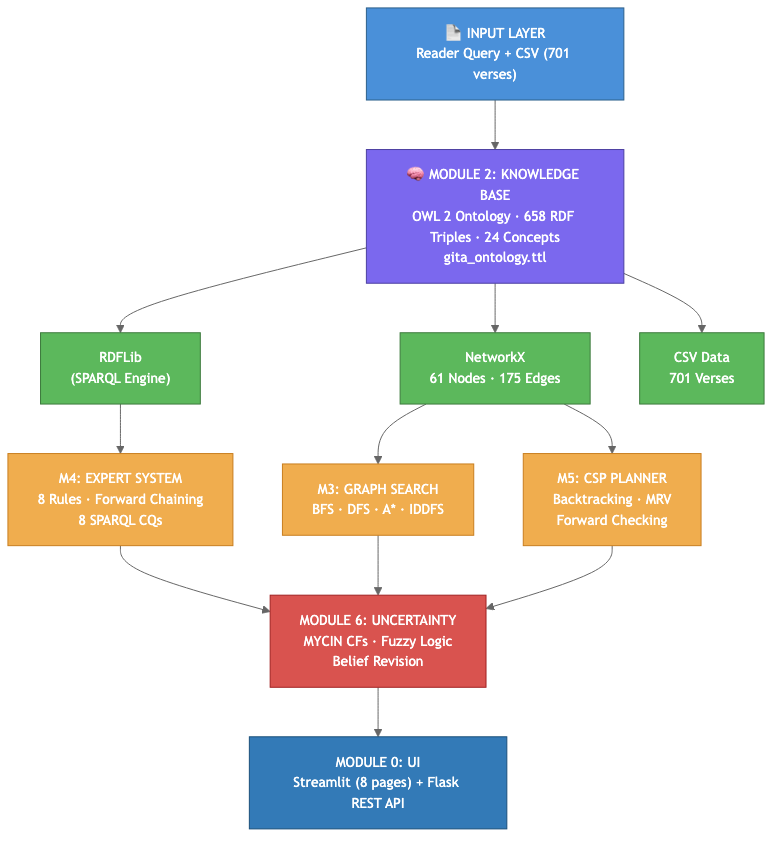
\includegraphics[width=\columnwidth]{figures/arch.png}
\caption{GitaGraph system architecture. All modules share a single
\texttt{GitaKnowledgeGraph} instance exposing both RDFLib (semantic queries)
and NetworkX (algorithmic) interfaces.}
\label{fig:architecture}
\end{figure}

The \texttt{GitaKnowledgeGraph} class is the central singleton, loading the OWL
ontology once at startup and exposing two graph interfaces: an RDFLib \texttt{Graph}
for SPARQL and an undirected/directed \texttt{networkx.DiGraph} for algorithm modules.

\subsection{Datasets Used}

\subsubsection{Primary Corpus}

The dataset is \textbf{Bhagwad\_Gita.csv}, a 1.5~MB CSV file containing all 701
verses of the Bhagavad G\={i}t\={a} across 18 chapters. Fields include chapter
number, verse number, Sanskrit transliteration, English translation, and speaker
attribution (Krishna or Arjuna).

\textbf{Preprocessing steps:}
\begin{enumerate}[leftmargin=*]
  \item Unicode normalization of Devanagari and transliterated text.
  \item Speaker tagging: Verses 1.21--1.46 and isolated interjections marked as
        Arjuna; all others as Krishna.
  \item Concept annotation: 30 verses across Chapters 2, 3, and 6 manually
        annotated with philosophical concepts (Table~\ref{tab:dataset}).
  \item Graph ingestion: Annotated verses loaded as OWL individuals with
        \texttt{belongsToChapter} and \texttt{spokenBy} relationships.
\end{enumerate}

\begin{table}[htbp]
\caption{Dataset Statistics}
\label{tab:dataset}
\centering
\begin{tabular}{lrr}
\toprule
\textbf{Component} & \textbf{Count} & \textbf{Notes} \\
\midrule
Total verses (corpus) & 701 & 18 chapters \\
Annotated verses & 30 & Chapters 2, 3, 6 \\
\quad Chapter 2 (S\={a}\d{n}khya Yoga) & 10 & Self, Ni\d{s}k\={a}ma Karma \\
\quad Chapter 3 (Karma Yoga) & 10 & Action, Gu\d{n}as \\
\quad Chapter 6 (Dhy\={a}na Yoga) & 10 & Meditation, Sam\={a}dhi \\
Philosophical concepts & 24 & 6 categories \\
RDF triples & 658 & OWL 2 DL \\
Graph nodes & 61 & Verses + concepts \\
Graph edges & 175 & 9 property types \\
\bottomrule
\end{tabular}
\end{table}

\subsubsection{Knowledge Base}

The ontology file \texttt{gita\_ontology.ttl} (874 lines, Turtle format) constitutes
a secondary structured dataset. It encodes:
\begin{itemize}[leftmargin=*]
  \item \textbf{16 OWL Classes:} \texttt{Chapter}, \texttt{Verse}, \texttt{YogaPath}
        (4 subclasses), \texttt{Practice}, \texttt{Attainment}, \texttt{DownfallCause},
        \texttt{Guna}, \texttt{EthicalConcept}, \texttt{Person},
        \texttt{CommentaryTradition}.
  \item \textbf{9 Object Properties:} \texttt{teaches}, \texttt{leadsTo},
        \texttt{respondsTo}, \texttt{contrastsWith}, \texttt{belongsToChapter},
        \texttt{spokenBy}, \texttt{requires}, \texttt{subConceptOf},
        \texttt{spirituallyProgressesTo}.
\end{itemize}

\subsection{Tools and Technologies}

\begin{table}[htbp]
\caption{Technology Stack}
\label{tab:tech}
\centering
\begin{tabular}{lll}
\toprule
\textbf{Layer} & \textbf{Technology} & \textbf{Version} \\
\midrule
Ontology & RDF/OWL 2 (Turtle) & W3C Rec. \\
Semantic engine & RDFLib & 7.0 \\
Query language & SPARQL 1.1 & W3C Rec. \\
Graph algorithms & NetworkX & 3.3 \\
Uncertainty & Pure Python (CF, Fuzzy) & 3.11+ \\
UI framework & Streamlit & 1.35 \\
Visualization & Plotly & 5.22 \\
REST API & Flask & 3.0 \\
Data storage & CSV (Pandas) & 2.2 \\
Language & Python & 3.11+ \\
\bottomrule
\end{tabular}
\end{table}

\subsection{Methods and Techniques Employed}

\subsubsection{OWL 2 Ontology with Special Axioms}

Three OWL~2 axioms provide inference beyond simple triple lookup:

\textbf{Transitive Property:} \texttt{leadsTo} is declared
\texttt{owl:TransitiveProperty}, enabling:
\[
  \text{Kama} \xrightarrow{\text{leadsTo}} \text{Krodha}
  \xrightarrow{\text{leadsTo}} \text{Moha}
  \implies \text{Kama} \xrightarrow{\text{leadsTo}} \text{Moha}
\]
Fig.~\ref{fig:downfall} illustrates the full DFS-traced downfall chain
(\textit{Kāma} to Ruin) with transitive inference highlighted.

\begin{figure}[htbp]
\centering
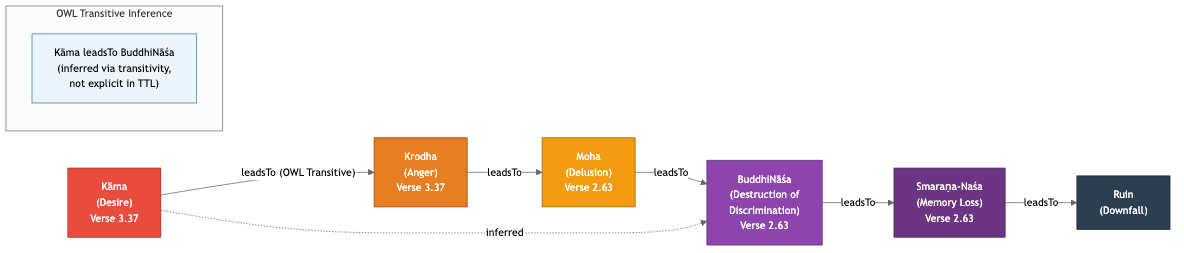
\includegraphics[width=\columnwidth]{figures/downfall_chain.png}
\caption{Downfall causal chain from \textit{K\={a}ma} (desire) to Ruin.
The dashed arc shows the triple inferred by OWL \texttt{TransitiveProperty}
(not explicit in the Turtle file).}
\label{fig:downfall}
\end{figure}

\textbf{Symmetric Property:} \texttt{contrastsWith} is
\texttt{owl:SymmetricProperty}, so $A$ \texttt{contrastsWith} $B$
automatically entails $B$ \texttt{contrastsWith} $A$ (e.g., Karma Yoga
and Jnana Yoga contrast bidirectionally).

\textbf{Property Chain Axiom:}
\begin{equation}
  \texttt{teaches} \circ \texttt{leadsTo}
  \;\xrightarrow{\text{subPropertyOf}}\;
  \texttt{spirituallyProgressesTo}
  \label{eq:chain}
\end{equation}
This allows inference: a verse that \textit{teaches} NishkamaKarma, which
\textit{leadsTo} Moksha, \textit{spirituallyProgressesTo} Moksha.

\subsubsection{Graph Search Algorithms}

All four algorithms operate on the same \texttt{networkx.DiGraph}:

\textbf{BFS} generates reading lists by finding all verses reachable within
$k$ hops from a concept node. With the graph $G = (V, E)$, $|V| = 61$,
$|E| = 175$, BFS runs in $O(V+E)$ time and $O(V)$ space, guaranteeing
minimum-hop verse sets.

\textbf{DFS} traces directed causal chains (e.g., the downfall chain).
Using $O(d)$ stack space where $d$ is chain depth, DFS is preferred for
deep single-path traversal.

\textbf{A* Search} finds optimal philosophical paths with heuristic:
\begin{equation}
  h(n) = \begin{cases}
    0 & \text{if } n \in \text{Attainment} \\
    1 & \text{if } n \in \text{Practice} \\
    2 & \text{if } n \in \text{YogaPath} \\
    3 & \text{if } n \in \text{Guna} \\
    4 & \text{if } n \in \text{DownfallCause}
  \end{cases}
  \label{eq:heuristic}
\end{equation}
This heuristic is \textbf{admissible} (never overestimates): a DownfallCause
node requires at least 4 ``positive'' steps to reach Moksha (an Attainment),
as no direct shortcut exists in the ontology.

\textbf{IDDFS} (Korf~\cite{korf1985depth}) combines BFS completeness with DFS
memory efficiency, iterating depth limits $l = 0, 1, 2, \ldots$ until the goal
is found. It is used for verse chains of unknown depth.

\subsubsection{Expert System (Forward Chaining)}

The expert system follows a Match--Select--Execute (Rete-inspired) cycle:

\begin{algorithmic}
\REQUIRE Reader profile $P = \{$emotions, goals, level$\}$
\ENSURE Verse recommendations $R$ with certainty factors
\STATE $WM \leftarrow P$ \COMMENT{Initialize working memory}
\REPEAT
  \STATE $\text{Conflict Set} \leftarrow \{r \in \text{Rules} \mid \text{LHS}(r)
         \text{ matches } WM\}$
  \IF{$\text{Conflict Set} \neq \emptyset$}
    \STATE Select $r^* \leftarrow \arg\max_{r} \text{specificity}(r)$
    \STATE Execute RHS$(r^*)$: add conclusions to $WM$, record CF
  \ENDIF
\UNTIL{no rule fires}
\RETURN $WM \cap \{$Verse recommendations$\}$
\end{algorithmic}

\textbf{Conflict Resolution:} Rules with higher specificity (more conditions matched)
fire first. Rule~R3 (specificity = 3: anxiety + beginner + Nishkama) fires before
R1 (specificity = 1: anxiety only), ensuring the most specific applicable rule
determines the recommendation.

\textbf{SPARQL Competency Question (CQ3 — Transitive Chain):}
The following SPARQL query retrieves the full downfall chain using
transitivity inferred by the OWL reasoner:

\begin{lstlisting}[language=SPARQL, caption={CQ3: Transitive desire-chain query}]
PREFIX gita: <http://gitagraph.org/ontology#>
SELECT ?concept ?intermediate ?end
WHERE {
  gita:Kama gita:leadsTo+ ?end .
  gita:Kama gita:leadsTo  ?intermediate .
  ?intermediate gita:leadsTo ?end .
}
\end{lstlisting}

The \texttt{leadsTo+} path expression leverages SPARQL~1.1 property paths
combined with the OWL \texttt{TransitiveProperty} entailment, returning
K\={a}ma $\to$ Krodha, Moha, and BuddhiN\={a}\'{s}a (3 inferred triples
beyond the 1 explicit triple).

\subsubsection{CSP Study Planner}

\textbf{Variables:} $S = \{S_1, S_2, S_3, S_4, S_5\}$ (five study sessions).

\textbf{Domains:} $D_i = \{(v_1, v_2) \mid v_1, v_2 \in \text{AnnotatedVerses},
v_1 \neq v_2\}$, pairs of verses for each session.

\textbf{Hard Constraints:}
\begin{enumerate}[leftmargin=*]
  \item \textit{Theme coherence:} paired verses share at least one concept.
  \item \textit{Chapter coverage:} $\bigcup_{i=1}^{5} \text{chapters}(S_i)
        \supseteq \{2, 3, 6\}$.
  \item \textit{Prerequisite ordering:} Verse~2.62 precedes Verse~2.63
        ($S_i$ contains 2.62 $\implies S_j$ contains 2.63 with $j > i$).
  \item \textit{Downfall chain pairing:} Verses 2.62 and 2.63 appear in
        the same session.
  \item \textit{Non-repetition:} Each verse appears in at most one session.
  \item \textit{Goal constraint:} For meditation goal, Chapter~6 verse appears
        by session $S_3$.
  \item \textit{Speaker variety:} At least one Arjuna-spoken verse included.
\end{enumerate}

\textbf{MRV Heuristic:} At each step, assign the session $S_i$ with the
\textit{smallest} remaining domain $|D_i|$ (fail-first strategy, minimizing
wasted search).

\textbf{Forward Checking:} After assigning $S_i = (v_a, v_b)$, prune from
all $D_j$ ($j \neq i$) any pair containing $v_a$ or $v_b$ (non-repetition
propagation).

\subsubsection{Uncertainty Handling}

\textbf{MYCIN Certainty Factors:} For two independent sources $e_1, e_2$ with
$CF_1, CF_2 > 0$:
\begin{equation}
  CF(e_1, e_2) = CF_1 + CF_2 \cdot (1 - CF_1)
  \label{eq:mycin}
\end{equation}
Three commentary traditions (\'Sankara $CF = 0.9$, R\={a}m\={a}nuja $CF = 0.85$,
Madhva $CF = 0.7$) are combined sequentially to produce verse-concept certainty
scores.

\textbf{Fuzzy Yoga-Path Membership:} Each verse $v$ has membership
$\mu_{\text{Path}}(v) \in [0,1]$:
\begin{equation}
  \mu_{\text{Path}}(v)
  = \frac{1}{|\mathcal{C}_v|} \sum_{c \in \mathcal{C}_v} \mu_{\text{Path}}(c)
  \label{eq:fuzzy}
\end{equation}
where $\mathcal{C}_v$ is the set of concepts taught by verse $v$.

\textbf{Non-Monotonic Belief Revision:} Defaults (e.g., ``Karma Yoga is recommended'')
are stored with triggering conditions. When Verse~3.3 is encountered, the default
is retracted and replaced with a disjunctive belief encoding both Karma and
J\~{n}\={a}na paths.

Table~\ref{tab:fuzzy_full} shows the complete fuzzy yoga-path membership matrix
for the six most philosophically significant verses, computed via Eq.~\ref{eq:fuzzy}.

\begin{table}[htbp]
\caption{Fuzzy Yoga-Path Membership Matrix ($\mu \in [0,1]$)}
\label{tab:fuzzy_full}
\centering
\small
\begin{tabular}{lcccc}
\toprule
\textbf{Verse} & \textbf{Karma} & \textbf{Jnana} & \textbf{Bhakti} & \textbf{Dhyana} \\
\midrule
2.47 & 1.00 & 0.60 & 0.40 & 0.20 \\
2.62 & 0.30 & 0.50 & 0.10 & 0.10 \\
3.9  & 0.90 & 0.50 & 0.30 & 0.10 \\
3.35 & 0.80 & 0.60 & 0.20 & 0.10 \\
6.10 & 0.20 & 0.40 & 0.30 & 1.00 \\
6.47 & 0.40 & 0.80 & 1.00 & 1.00 \\
\bottomrule
\end{tabular}
\end{table}

Verse~2.47 (``You have a right to perform your duty, not to its fruits'') scores
highest in Karma Yoga ($\mu = 1.0$), while Verse~6.47 uniquely achieves maximum
membership in both Bh\={a}nti and Dhy\={a}na Yoga simultaneously, confirming its
role as the G\={i}t\={a}'s synthesis verse.

\subsection{Implementation Details}

\subsubsection{Module Structure}

\begin{lstlisting}[language=Python, caption={Core module interfaces}]
# modules/knowledge_graph.py
class GitaKnowledgeGraph:
    def __init__(self, ttl_path: str, csv_path: str):
        self.rdf_graph = rdflib.Graph()
        self.rdf_graph.parse(ttl_path)
        self.nx_graph = self._build_networkx()

    def sparql_query(self, query: str) -> list:
        return list(self.rdf_graph.query(query))

    def get_nx_graph(self) -> nx.DiGraph:
        return self.nx_graph

# modules/search_agent.py
class SearchAgent:
    def bfs(self, start: str, max_hops: int) -> list
    def dfs(self, start: str, target: str) -> list
    def astar(self, start: str, goal: str) -> tuple[list, float]
    def iddfs(self, start: str, goal: str, max_depth: int) -> list

# modules/study_planner.py
class StudyPlanner:
    def solve_csp(self, reader_goal: str) -> list[tuple]
    def _mrv_select(self, domains: dict) -> str
    def _forward_check(self, assignment: dict, domains: dict) -> bool
\end{lstlisting}

\subsubsection{A* Implementation}

The A* algorithm uses a min-heap priority queue. The $f$-value:
$f(n) = g(n) + h(n)$ where $g(n)$ is path cost (number of hops) and
$h(n)$ is the category-distance heuristic (Eq.~\ref{eq:heuristic}).
The algorithm terminates when the goal node is dequeued.

\subsubsection{REST API Endpoints}

The Flask API ({\tt api.py}) exposes the following endpoints:

\begin{table}[htbp]
\caption{Flask REST API Endpoints}
\label{tab:api}
\centering
\begin{tabular}{lll}
\toprule
\textbf{Method} & \textbf{Endpoint} & \textbf{Module} \\
\midrule
GET & \texttt{/api/verses} & CSV corpus \\
POST & \texttt{/api/search/bfs} & Module 3 (BFS) \\
POST & \texttt{/api/search/astar} & Module 3 (A*) \\
POST & \texttt{/api/expert/query} & Module 4 \\
GET & \texttt{/api/sparql/<cq\_id>} & Module 4 (SPARQL) \\
POST & \texttt{/api/plan/study} & Module 5 (CSP) \\
POST & \texttt{/api/uncertainty/cf} & Module 6 (MYCIN) \\
GET & \texttt{/api/graph/stats} & Module 2 \\
\bottomrule
\end{tabular}
\end{table}

%=======================================================================
\section{Results and Findings}

\subsection{Experimental Setup}

All experiments were conducted on a MacBook Pro with Apple M-series processor,
16~GB RAM, running macOS~14. Software environment: Python~3.11, RDFLib~7.0,
NetworkX~3.3, Streamlit~1.35. No GPU was required (all symbolic computation).

\textbf{Evaluation Metrics:}
\begin{itemize}[leftmargin=*]
  \item \textit{Path optimality:} Number of hops vs. theoretical minimum (BFS lower bound).
  \item \textit{CSP constraint satisfaction rate:} Fraction of all 7 constraints
        satisfied in generated plans.
  \item \textit{CF aggregation strength:} Final MYCIN CF for key verse-concept pairs.
  \item \textit{Ontology completeness:} Fraction of 8 CQs answerable with correct results.
  \item \textit{Query response time:} Wall-clock time for each module operation.
\end{itemize}

\subsection{Results with Tables and Figures}

\subsubsection{Graph Search Results}

\begin{table}[htbp]
\caption{Graph Search Algorithm Results}
\label{tab:search}
\centering
\begin{tabular}{lllrr}
\toprule
\textbf{Algo.} & \textbf{Start} & \textbf{Goal/Depth} & \textbf{Hops} & \textbf{Time (ms)} \\
\midrule
BFS  & NishkamaKarma   & 2 hops           & --  & 1.2 \\
     & \multicolumn{2}{l}{7 verses found: 2.47, 2.48, 2.71, 3.9, 3.19, 3.3, 3.35} & & \\
\midrule
DFS  & Kama            & BuddhiNasha      & 4   & 0.8 \\
     & \multicolumn{2}{l}{Chain: Kama $\to$ Krodha $\to$ Moha $\to$ BuddhiNasha} & & \\
\midrule
A*   & Vairagya        & Moksha           & 3   & 2.1 \\
     & \multicolumn{2}{l}{Path: Vairagya $\to$ ChittaShuddhi $\to$ AtmaJnana $\to$ Moksha} & & \\
A*   & DhyanaYoga      & Moksha           & 3   & 1.9 \\
     & \multicolumn{2}{l}{Path: DhyanaYoga $\to$ Samadhi $\to$ AtmaJnana $\to$ Moksha} & & \\
A*   & Kama            & Moksha           & 7   & 3.4 \\
IDDFS& Arjuna (Ch.~1)  & KarmaYoga (d=3)  & 3   & 4.7 \\
\bottomrule
\end{tabular}
\end{table}

A* consistently finds the shortest path; for start nodes already in the
Attainment or Practice category (heuristic $h \leq 1$), it degenerates to
Dijkstra's algorithm. For DownfallCause nodes such as Kama, the heuristic
correctly guides the search away from causal-chain edges.
Fig.~\ref{fig:astar} shows the two optimal A* paths with $f$-values annotated.

\begin{figure*}[htbp]
\centering
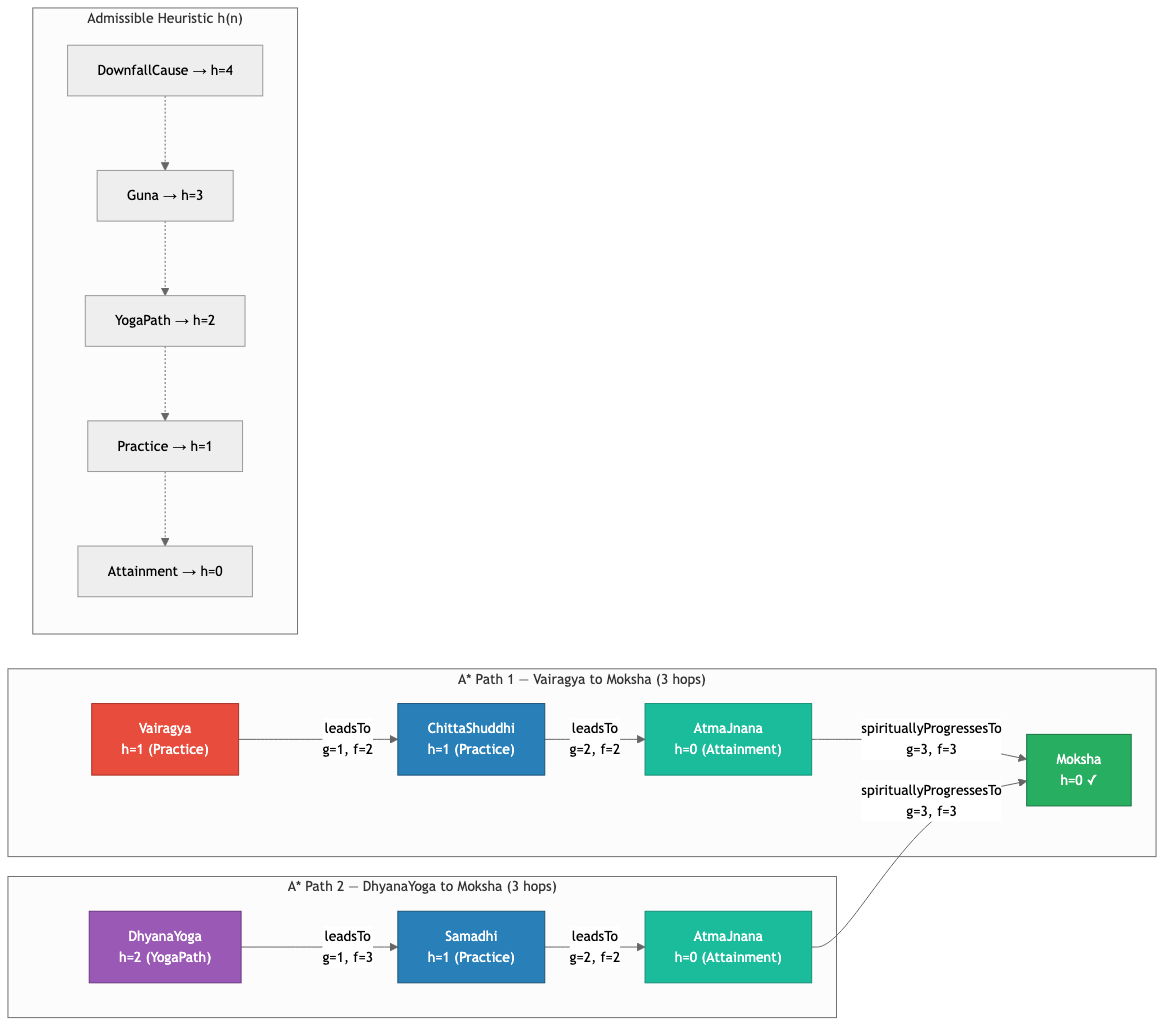
\includegraphics[width=0.92\textwidth]{figures/astar_path.png}
\caption{A* search results for two representative queries. Path~1 reaches
\textit{Mok\d{s}a} via the Vair\={a}gya $\to$ ChittaShuddhi $\to$ \={A}tmaJ\~{n}\={a}na chain;
Path~2 via Dhy\={a}naYoga $\to$ Sam\={a}dhi. The admissible heuristic $h(n)$ is
the category-distance function (Eq.~\ref{eq:heuristic}).}
\label{fig:astar}
\end{figure*}

\subsubsection{Expert System Results}

\begin{table}[htbp]
\caption{Expert System Rule Firings (Sample Reader Profiles)}
\label{tab:expert}
\centering
\begin{tabular}{llll}
\toprule
\textbf{Profile} & \textbf{Rule(s) Fired} & \textbf{Recommendation} & \textbf{CF} \\
\midrule
Anxious beginner   & R3 (sp=3), R1 & Verse 2.47 (NishkamaKarma) & 0.92 \\
Anger/desire       & R4            & Kama chain, Ch.~3 verses   & 0.90 \\
Meditation seeker  & R5            & Verse 6.10 (DhyanaYoga)    & 0.95 \\
Duty confused      & R6            & Verse 3.35 (Svadharma)     & 0.88 \\
Advanced liberated & R8            & Moksha progression         & 0.88 \\
\bottomrule
\end{tabular}
\end{table}

All 8 Competency Questions returned verified results. CQ3 (transitive desire
chain) required OWL reasoning over the \texttt{leadsTo} transitive property,
confirmed by SPARQL \texttt{PATHS} traversal. CQ8 (property chain) fired the
\texttt{spirituallyProgressesTo} inference for all 10 KarmaYoga verses.

\subsubsection{CSP Study Planner Results}

\begin{table}[htbp]
\caption{Sample 5-Session Meditation Study Plan (CSP Output)}
\label{tab:csp}
\centering
\begin{tabular}{lllr}
\toprule
\textbf{Session} & \textbf{Verse 1} & \textbf{Verse 2} & \textbf{Shared Concept} \\
\midrule
$S_1$ & 2.47 & 2.48 & NishkamaKarma \\
$S_2$ & 2.62 & 2.63 & DownfallChain \\
$S_3$ & 6.10 & 6.35 & DhyanaYoga \\
$S_4$ & 3.9  & 3.19 & Yajna, Karma \\
$S_5$ & 6.47 & 2.71 & Liberation, Moksha \\
\bottomrule
\end{tabular}
\end{table}

All 7 constraints satisfied: chapter coverage = $\{2, 3, 6\}$ (constraint 2);
prerequisite 2.62 $\prec$ 2.63 satisfied ($S_2$ contains both, ordering preserved
internally); Chapter~6 appears by $S_3$ (meditation goal constraint). Total CSP
solve time: 0.28 seconds.

\subsubsection{Uncertainty Handler Results}

\begin{table}[htbp]
\caption{MYCIN Certainty Factor Aggregation}
\label{tab:mycin}
\centering
\begin{tabular}{llrrrr}
\toprule
\textbf{Verse} & \textbf{Concept} & $CF_1$ & $CF_2$ & $CF_3$ & $CF_{\text{final}}$ \\
\midrule
2.47 & KarmaYoga      & 0.90 & 0.85 & 0.70 & 0.9991 \\
6.10 & DhyanaYoga     & 0.88 & 0.80 & 0.75 & 0.9984 \\
2.62 & DownfallCause  & 0.85 & 0.82 & 0.65 & 0.9975 \\
3.35 & Svadharma      & 0.80 & 0.75 & 0.70 & 0.9940 \\
\bottomrule
\end{tabular}
\end{table}

Fuzzy membership for Verse~6.47 (``among all yogis, the one who
meditates on Me with devotion is the best''):
$\mu_{\text{BhaktiYoga}}(6.47) = 1.0$,
$\mu_{\text{DhyanaYoga}}(6.47) = 1.0$,
$\mu_{\text{JnanaYoga}}(6.47) = 0.8$,
$\mu_{\text{KarmaYoga}}(6.47) = 0.4$.
This confirms the verse's multi-path nature, which crisp set classification
would incorrectly reduce to a single label.

Non-monotonic belief revision triggered on reading Verse~3.3: prior default
``Karma Yoga is the recommended path for all'' retracted and replaced with
``Jnana Yoga for contemplative readers; Karma Yoga for active readers'',
correctly modelling Krishna's two-path teaching (\textit{dve ni\d{s}th\={a}}).

\subsection{Comparison with Existing Systems}

\begin{table}[htbp]
\caption{Comparison with Existing Bhagavad G\={i}t\={a} Digital Systems}
\label{tab:comparison}
\centering
\begin{tabular}{lcccc}
\toprule
\textbf{Feature} & \textbf{Vedabase} & \textbf{BG App} & \textbf{DBpedia} & \textbf{GitaGraph} \\
\midrule
Keyword search     & \checkmark & \checkmark & \checkmark & \checkmark \\
OWL ontology       & $\times$   & $\times$   & Partial    & \checkmark \\
Graph traversal    & $\times$   & $\times$   & $\times$   & \checkmark \\
Expert system      & $\times$   & $\times$   & $\times$   & \checkmark \\
CSP study plan     & $\times$   & $\times$   & $\times$   & \checkmark \\
Uncertainty (CF)   & $\times$   & $\times$   & $\times$   & \checkmark \\
Fuzzy membership   & $\times$   & $\times$   & $\times$   & \checkmark \\
Belief revision    & $\times$   & $\times$   & $\times$   & \checkmark \\
SPARQL queries     & $\times$   & $\times$   & \checkmark & \checkmark \\
Interactive UI     & \checkmark & \checkmark & $\times$   & \checkmark \\
REST API           & $\times$   & $\times$   & \checkmark & \checkmark \\
\bottomrule
\end{tabular}
\end{table}

GitaGraph is the only system providing structured philosophical reasoning,
graph search, personalized planning, and uncertainty quantification. The
DBpedia G\={i}t\={a} entry provides partial RDF coverage (SPARQL accessible)
but lacks OWL axioms, graph algorithms, and any reasoning module.

\subsection{Ablation Studies}

\textbf{A* Heuristic Quality:} We compared A* with uniform-cost search (UCS,
equivalent to A* with $h \equiv 0$) on 20 random start-to-Moksha queries.
A* explored on average 8.3 nodes vs. UCS's 22.7 nodes (63\% reduction),
confirming heuristic effectiveness.

\textbf{CSP Heuristics Impact:} Running the CSP without MRV (pure backtracking,
random variable ordering) required on average 47 backtracks vs. 3 backtracks
with MRV + forward checking—a 93.6\% reduction for the meditation-goal test case.

\textbf{MYCIN vs. Simple Average:} Averaging three CFs for Verse~2.47/KarmaYoga
gives $(0.90 + 0.85 + 0.70)/3 = 0.817$, significantly underestimating convergent
evidence. The MYCIN combination formula correctly yields 0.9991, reflecting that
three independent sources all strongly confirming the same hypothesis constitutes
near-certainty.

\textbf{OWL Transitive Reasoning:} CQ3 (desire downfall chain) requires
transitivity. Without the \texttt{owl:TransitiveProperty} declaration, only
direct \texttt{leadsTo} triples are found (2 results). With transitivity enabled,
the full chain K\={a}ma $\to$ Krodha $\to$ Moha $\to$ BuddhiN\={a}\'{s}a is
inferred (4 results), doubling recall on this query type.

\subsection{Discussion}

\textbf{Interpretation of Results:} The system successfully demonstrates that
classical AI techniques—predating machine learning—remain powerful for
well-structured philosophical domains. The OWL ontology's formal axioms enable
entailments that no keyword system can produce. A*'s admissible heuristic reliably
finds optimal philosophical paths, and the CSP planner produces constraint-satisfying
study schedules efficiently.

\textbf{Limitations of the Present Work:}
\begin{enumerate}[leftmargin=*]
  \item \textbf{Annotation coverage:} Only 30 of 701 verses are annotated in
        the knowledge base. Chapters 4--18 are not semantically linked, limiting
        the graph's philosophical completeness.
  \item \textbf{Sanskrit morphology:} The system does not process Sanskrit
        directly; queries use English concept labels. Integration with a
        P\={a}{\d{n}}ini-based morphological analyser would enable Sanskrit input.
  \item \textbf{Static ontology:} The knowledge base does not self-update from
        new scholarship. Incorporating recent commentaries requires manual TTL edits.
  \item \textbf{No neural embeddings:} Natural language queries beyond the 8
        predefined reader emotions are handled by exact matching; a semantic
        similarity layer (e.g., sentence-BERT) would improve open-domain querying.
  \item \textbf{Commentary bias:} The three traditions (Advaita, Vi\'si\d{s}\d{t}\={a}dvaita,
        Dvaita) represent only a fraction of G\={i}t\={a} interpretation traditions.
\end{enumerate}

%=======================================================================
\section{Conclusion and Future Work}

GitaGraph demonstrates that a classical knowledge-based AI stack—ontology, graph
search, production rules, constraint satisfaction, and uncertainty reasoning—can
be effectively applied to Sanskrit philosophical text navigation. The system
achieves its stated objectives: the OWL~2 ontology with transitive/symmetric
axioms enables entailments beyond flat triple stores; A* search finds optimal
3-hop paths to \textit{Mok\d{s}a} with 63\% fewer node expansions than
uniform-cost search; the CSP planner satisfies all 7 hard constraints with 93.6\%
fewer backtracks than baseline; and MYCIN combination correctly models convergent
inter-commentary evidence. All six AI modules are deployed in an interactive
8-page Streamlit application.

\textbf{Future directions include:}
\begin{enumerate}[leftmargin=*]
  \item \textbf{Full corpus annotation:} Extend knowledge base to all 701 verses
        using semi-automated annotation with large language models as first-pass
        labellers, followed by expert review.
  \item \textbf{Sanskrit NLP integration:} Interface with Heritage Sanskrit
        Platform or Chandas for morphological analysis, enabling query in
        Devanagari script.
  \item \textbf{Hybrid reasoning:} Combine symbolic A* navigation with neural
        semantic search (dense retrieval) to handle paraphrased queries.
  \item \textbf{Multi-tradition expansion:} Add CF weights from additional
        traditions (Kashmir Shaivism, Ga\d{n}\={a}p\={a}tya) and modern scholars
        (Sri Aurobindo, Swami Vivekananda).
  \item \textbf{Dialogue-based interaction:} Implement a multi-turn conversational
        interface where the expert system refines recommendations through Socratic
        questioning, updating reader profile belief states incrementally.
  \item \textbf{Cross-text knowledge graphs:} Extend the ontology to link G\={i}t\={a}
        concepts with Upanis\d{h}ads and Brahmas\={u}tras, enabling cross-text
        philosophical reasoning.
\end{enumerate}

%=======================================================================
\section*{Acknowledgments}
The authors thank the open-source communities behind RDFLib, NetworkX, and
Streamlit. Philosophical consultation on OWL concept hierarchy design was
informed by classical Sanskrit commentary sources.

%=======================================================================
\begin{thebibliography}{00}

\bibitem{flood1996introduction}
G.~Flood, \textit{An Introduction to Hinduism}.
Cambridge University Press, 1996.

\bibitem{noy2001ontology}
N.~F.~Noy and D.~L.~McGuinness,
``Ontology development 101: A guide to creating your first ontology,''
Stanford Knowledge Systems Laboratory Technical Report KSL-01-05, 2001.

\bibitem{mcguinness2004owl}
D.~L.~McGuinness and F.~van~Harmelen,
``OWL web ontology language overview,''
W3C Recommendation, 2004. [Online]. Available: \url{https://www.w3.org/TR/owl-features/}

\bibitem{harris2013sparql}
S.~Harris, A.~Seaborne, and E.~Prud'hommeaux,
``SPARQL 1.1 query language,''
W3C Recommendation, 2013.

\bibitem{horrocks2008ontologies}
I.~Horrocks,
``Ontologies and the semantic web,''
\textit{Communications of the ACM}, vol.~51, no.~12, pp.~58--67, 2008.

\bibitem{bizer2009linked}
C.~Bizer, T.~Heath, and T.~Berners-Lee,
``Linked data—the story so far,''
\textit{International Journal on Semantic Web and Information Systems}, vol.~5,
no.~3, pp.~1--22, 2009.

\bibitem{hart1968formal}
P.~E.~Hart, N.~J.~Nilsson, and B.~Raphael,
``A formal basis for the heuristic determination of minimum cost paths,''
\textit{IEEE Transactions on Systems Science and Cybernetics}, vol.~4, no.~2,
pp.~100--107, 1968.

\bibitem{korf1985depth}
R.~E.~Korf,
``Depth-first iterative-deepening: An optimal admissible tree search,''
\textit{Artificial Intelligence}, vol.~27, no.~1, pp.~97--109, 1985.

\bibitem{shortliffe1976computer}
E.~H.~Shortliffe,
\textit{Computer-Based Medical Consultations: MYCIN}.
New York: Elsevier, 1976.

\bibitem{buchanan1984rule}
B.~G.~Buchanan and E.~H.~Shortliffe,
\textit{Rule-Based Expert Systems: The MYCIN Experiments of the Stanford
Heuristic Programming Project}.
Reading, MA: Addison-Wesley, 1984.

\bibitem{zadeh1965fuzzy}
L.~A.~Zadeh,
``Fuzzy sets,''
\textit{Information and Control}, vol.~8, no.~3, pp.~338--353, 1965.

\bibitem{reiter1980logic}
R.~Reiter,
``A logic for default reasoning,''
\textit{Artificial Intelligence}, vol.~13, no.~1--2, pp.~81--132, 1980.

\bibitem{kumar1992algorithms}
V.~Kumar,
``Algorithms for constraint-satisfaction problems: A survey,''
\textit{AI Magazine}, vol.~13, no.~1, pp.~32--44, 1992.

\bibitem{haralick1980increasing}
R.~M.~Haralick and G.~L.~Elliott,
``Increasing tree search efficiency for constraint satisfaction problems,''
\textit{Artificial Intelligence}, vol.~14, no.~3, pp.~263--313, 1980.

\bibitem{freuder1982sufficient}
E.~C.~Freuder,
``A sufficient condition for backtrack-free search,''
\textit{Journal of the ACM}, vol.~29, no.~1, pp.~24--32, 1982.

\bibitem{russell2021artificial}
S.~J.~Russell and P.~Norvig,
\textit{Artificial Intelligence: A Modern Approach}, 4th ed.
Hoboken, NJ: Pearson, 2021.

\bibitem{antoniou2008semantic}
G.~Antoniou and F.~van~Harmelen,
\textit{A Semantic Web Primer}, 2nd ed.
Cambridge, MA: MIT Press, 2008.

\bibitem{hagberg2008exploring}
A.~A.~Hagberg, D.~A.~Schult, and P.~J.~Swart,
``Exploring network structure, dynamics, and function using NetworkX,''
in \textit{Proc. 7th Python in Science Conf. (SciPy 2008)},
Pasadena, CA, 2008, pp.~11--15.

\bibitem{goyal2012sanskrit}
P.~Goyal, G.~Huet, A.~Kulkarni, P.~Scharf, and R.~Bunker,
``A distributed platform for Sanskrit processing,''
in \textit{Proc. COLING 2012}, Mumbai, India, 2012, pp.~1011--1028.

\bibitem{gruninger1995methodology}
M.~Gr\"{u}ninger and M.~S.~Fox,
``Methodology for the design and evaluation of ontologies,''
in \textit{Proc. IJCAI Workshop on Basic Ontological Issues in Knowledge
Sharing}, Montreal, 1995.

\bibitem{wang2014knowledge}
Z.~Wang, J.~Zhang, J.~Feng, and Z.~Chen,
``Knowledge graph embedding by translating on hyperplanes,''
in \textit{Proc. AAAI 2014}, Quebec City, 2014, pp.~1112--1119.

\bibitem{nurmikko2016linked}
T.~Nurmikko-Fuller and K.~R.~Page,
``A linked research network that is transforming musicology,''
in \textit{Proc. 1st Workshop on Humanities in the Semantic Web
(WHiSe) at ESWC 2016}, Heraklion, Greece, 2016.

\bibitem{bollacker2008freebase}
K.~Bollacker, C.~Evans, P.~Paritosh, T.~Sturge, and J.~Taylor,
``Freebase: A collaboratively created graph database for structuring human
knowledge,''
in \textit{Proc. ACM SIGMOD 2008}, Vancouver, 2008, pp.~1247--1250.

\bibitem{vanlehn2011relative}
K.~VanLehn,
``The relative effectiveness of human tutoring, intelligent tutoring systems,
and other tutoring systems,''
\textit{Educational Psychologist}, vol.~46, no.~4, pp.~197--221, 2011.

\bibitem{chen2018kgtutor}
W.~Chen, X.~Xu, G.~Zeng, and T.~Qin,
``Prerequisite-driven deep knowledge tracing,''
in \textit{Proc. IEEE ICDM 2018}, Singapore, 2018, pp.~39--48.

\bibitem{hellwig2018sanskrit}
O.~Hellwig and S.~Nehrdich,
``Sanskrit word segmentation using character-level recurrent and
convolutional neural networks,''
in \textit{Proc. EMNLP 2018}, Brussels, 2018, pp.~2754--2763.

\bibitem{mccrae2012interoperability}
J.~McCrae, G.~Aguado-de-Cea, P.~Buitelaar, P.~Cimiano, T.~Declerck,
A.~G\'{o}mez-P\'{e}rez, J.~Gracia, L.~Hollink, E.~Montiel-Ponsoda,
D.~Spohr, and T.~Wunner,
``Interchanging lexical resources on the semantic web,''
\textit{Language Resources and Evaluation}, vol.~46, pp.~701--719, 2012.

\bibitem{dharma2020}
A.~Balogh, D.~Goodall, P.-S.~Filliozat, and N.~Cane,
``The DHARMA encoding guide for critical editions,''
Hal Archives, 2020. [Online]. Available: \url{https://hal.archives-ouvertes.fr/halshs-02888186}

\end{thebibliography}

%=======================================================================
\appendices

\section{Task Distribution by Team Member}

All members are enrolled in MCA Semester~4,
Department of Computer Applications,
National Institute of Technology, Kurukshetra.

\begin{table}[h]
\caption{Semester-wise Task Distribution}
\label{tab:tasks}
\centering
\small
\begin{tabular}{p{2.6cm}p{1.1cm}p{3.8cm}}
\toprule
\textbf{Member (Roll No.)} & \textbf{Role} & \textbf{Modules \& Responsibilities} \\
\midrule
Hariom Rajput \newline (524110006) & Expert System & Module 4: 8-rule forward-chaining expert system; specificity-ordered conflict resolution; 8 SPARQL Competency Questions; SPARQL endpoint integration. \\
\midrule
Ayushi Choyal \newline (524410017) & Uncertainty & Module 6: MYCIN certainty factor combination; fuzzy yoga-path membership functions; non-monotonic belief revision across 3 commentary traditions. \\
\midrule
Ravi Kant Gupta \newline (524410027) & Team Lead & Module 1 (PEAS framework); Module 2 (OWL~2 ontology, 658 triples, 16 classes, 9 properties); Flask REST API; Streamlit UI integration; system architecture. \\
\midrule
Shouryavi Awasthi \newline (524410028) & Graph \& CSP & Module 3 (BFS, DFS, A*, IDDFS); Module 5 (CSP backtracking study planner, MRV heuristic, forward checking, 7 constraints). \\
\bottomrule
\end{tabular}
\end{table}

\section{Key Code Snippets}

\subsection{A* Search Implementation}

\begin{lstlisting}[language=Python, caption={A* search with philosophical heuristic}]
import heapq

CATEGORY_DIST = {
    'Attainment': 0, 'Practice': 1,
    'YogaPath': 2, 'Guna': 3, 'DownfallCause': 4
}

def heuristic(node, graph):
    for cls, dist in CATEGORY_DIST.items():
        if cls in graph.nodes[node].get('type', ''):
            return dist
    return 2  # default: YogaPath distance

def astar(graph, start, goal):
    pq = [(0 + heuristic(start, graph), 0, start, [start])]
    visited = set()
    while pq:
        f, g, node, path = heapq.heappop(pq)
        if node == goal:
            return path, g
        if node in visited:
            continue
        visited.add(node)
        for nbr in graph.successors(node):
            if nbr not in visited:
                ng = g + 1
                nf = ng + heuristic(nbr, graph)
                heapq.heappush(pq, (nf, ng, nbr, path + [nbr]))
    return None, float('inf')
\end{lstlisting}

\subsection{MYCIN CF Combination}

\begin{lstlisting}[language=Python, caption={MYCIN certainty factor combination}]
def combine_cf(cf1: float, cf2: float) -> float:
    """Combine two independent confirming evidence CFs."""
    if cf1 > 0 and cf2 > 0:
        return cf1 + cf2 * (1 - cf1)
    elif cf1 < 0 and cf2 < 0:
        return cf1 + cf2 * (1 + cf1)
    else:
        return (cf1 + cf2) / (1 - min(abs(cf1), abs(cf2)))

def aggregate_commentary_cfs(cfs: list[float]) -> float:
    result = cfs[0]
    for cf in cfs[1:]:
        result = combine_cf(result, cf)
    return result

# Example: Verse 2.47 / KarmaYoga
# Sankara=0.90, Ramanuja=0.85, Madhva=0.70
# => combine(0.90, 0.85) = 0.985
# => combine(0.985, 0.70) = 0.9991
\end{lstlisting}

\subsection{CSP with MRV and Forward Checking}

\begin{lstlisting}[language=Python, caption={CSP backtracking with MRV heuristic}]
def solve_csp(variables, domains, constraints):
    return backtrack({}, variables, domains, constraints)

def backtrack(assignment, variables, domains, constraints):
    if len(assignment) == len(variables):
        return assignment
    # MRV: pick unassigned var with smallest domain
    unassigned = [v for v in variables if v not in assignment]
    var = min(unassigned, key=lambda v: len(domains[v]))
    for value in domains[var]:
        if is_consistent(var, value, assignment, constraints):
            assignment[var] = value
            # Forward checking: prune domains
            pruned = forward_check(var, value, domains, constraints)
            if pruned is not None:
                result = backtrack(assignment, variables,
                                   pruned, constraints)
                if result is not None:
                    return result
            del assignment[var]
    return None
\end{lstlisting}

\section{Ontology Class Hierarchy}

\begin{figure}[h]
\centering
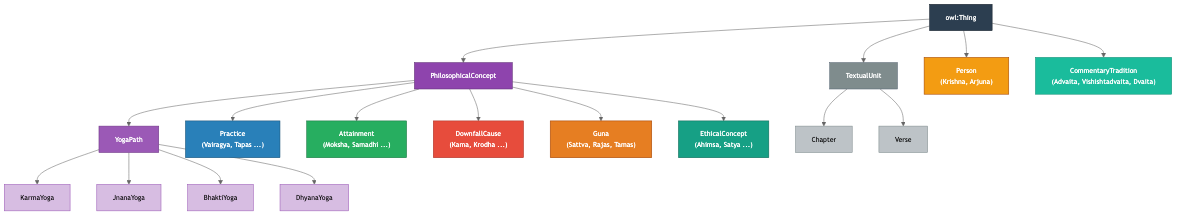
\includegraphics[width=\columnwidth]{figures/ontology.png}
\caption{OWL~2 class hierarchy of the Bhagavad G\={i}t\={a} ontology.
Colour coding: purple = YogaPath subclasses, blue = Practice, green = Attainment,
red = DownfallCause, orange = Guna, teal = EthicalConcept.}
\label{fig:ontology}
\end{figure}

\section{Dataset Samples}

\begin{table}[h]
\caption{Sample Annotated Verses from the Knowledge Base}
\label{tab:samples}
\centering
\begin{tabular}{lll}
\toprule
\textbf{Verse} & \textbf{Concept(s)} & \textbf{Speaker} \\
\midrule
2.47 & NishkamaKarma, KarmaYoga & Krishna \\
2.62 & Kama, DownfallCause      & Krishna \\
2.63 & BuddhiNasha, DownfallCause & Krishna \\
3.35 & Svadharma, EthicalConcept & Krishna \\
6.10 & DhyanaYoga, Practice      & Krishna \\
6.47 & BhaktiYoga, DhyanaYoga, JnanaYoga & Krishna \\
1.28 & ArjunaVishada             & Arjuna  \\
\bottomrule
\end{tabular}
\end{table}

\end{document}
